\section{Příklad 1}
% Jako parametr zadejte skupinu (A-H)
\prvniZadani{H}

\vspace{1cm}
\large{\textbf{Rešení (Metoda postupného zjednodušování):}}

%%% Krok 1
\begin{center}
\textbf{Krok 1} - Zjednodušení $U_1$ a $U_2$ podle vzorce pro sériově zapojené zdroje.
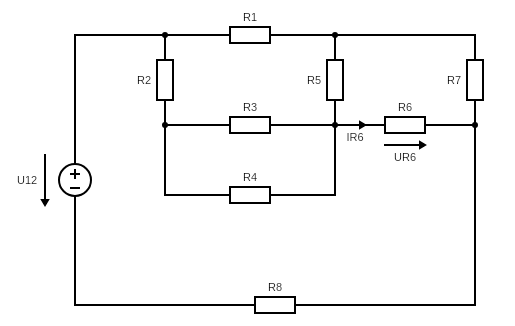
\includegraphics[scale=0.6,keepaspectratio]{fig/Pr1_steps/Pr1_step01.png} \\
\end{center}

\begin{gather*}
U_{12} = U_1 + U_2 = 135 + 80 = 215 V
\end{gather*}

\newpage

%%% Krok 2
\begin{center}
\textbf{Krok 2} - Zjednodušení $R_3$ a $R_4$ podle vzorce pro paralelně zapojené rezistory.
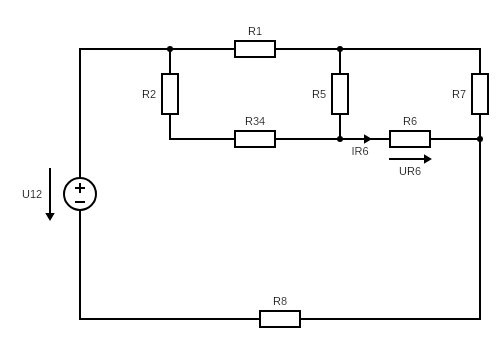
\includegraphics[scale=0.6,keepaspectratio]{fig/Pr1_steps/Pr1_step02.png} \\
\end{center}
\vspace{-0.3cm}

\begin{gather*}
R_{34} = \frac{R_3 \times R_4}{R_3 + R_4} = \frac{260 \times 310}{260 + 310} = 141,404 \Omega
\end{gather*}

%%% Krok 3
\vspace{1cm}
\begin{center}
\textbf{Krok 3} - Zjednodušení $R_2$ a $R_34$ podle vzorce pro sériově zapojené rezistory.
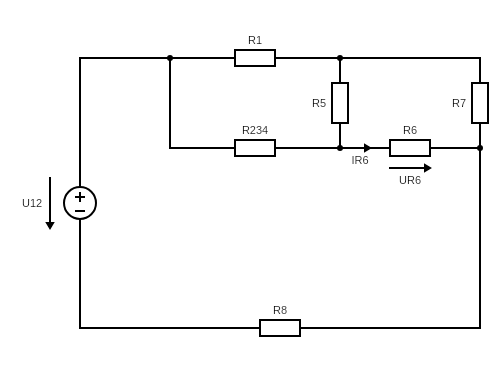
\includegraphics[scale=0.6,keepaspectratio]{fig/Pr1_steps/Pr1_step03.png} \\
\end{center}
\vspace{-0.3cm}

\begin{gather*}
R_{234} = R_2 + R_34 = 600 + 141,4040 = 741,404 \Omega
\end{gather*}

\newpage

%%% Krok 4
\begin{center}
\textbf{Krok 4} - Provedeme transfiguraci trojúhelník-hvězda.
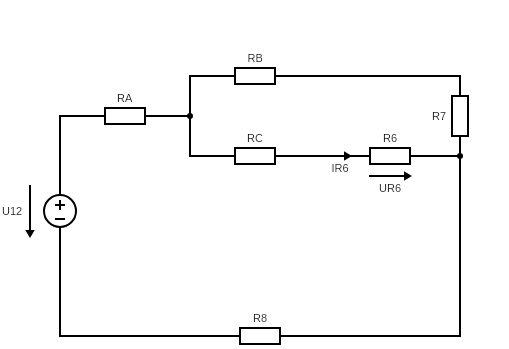
\includegraphics[scale=0.6,keepaspectratio]{fig/Pr1_steps/Pr1_step04.png} \\
\end{center}
\vspace{-0.3cm}

\begin{gather*}
\newline
R_A = \frac{R_1 \times R_{234}}{R_1 + R_5 + R_{234}} = \frac{680 \times 741,404}{680 + 575 + 741,404} = 252,5314 \Omega \\\\
\newline
\newline
R_B = \frac{R_1 \times R_5}{R_1 + R_5 + R_{234}} = \frac{680 \times 575}{680 + 575 + 741,404} = 195,8521 \Omega \\\\
\newline
\newline
R_C = \frac{R_5 \times R_{234}}{R_1 + R_5 + R_{234}} = \frac{575 \times 741,404}{680 + 575 + 741,404} = 213,5376 \Omega
\newline
\end{gather*}
\vspace{1cm}

%%% Krok 5
\begin{center}
\textbf{Krok 5} - Zjednodušíme sériově zapojené rezistory $R_B$, $R_7$ a $R_C$, $R_6$.
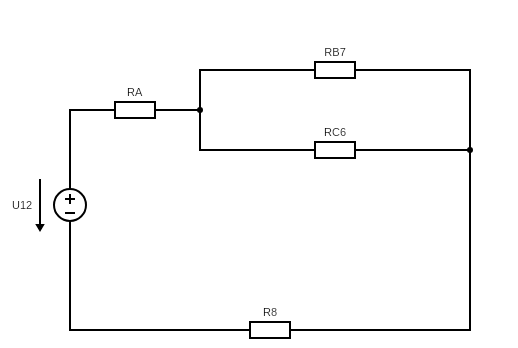
\includegraphics[scale=0.6,keepaspectratio]{fig/Pr1_steps/Pr1_step05.png} \\
\end{center}
\vspace{-0.3cm}

\begin{gather*}
R_{B7} = R_B + R_6 = 195,8521 + 355 = 550,8521 \Omega \\\\
R_{C6} = R_C + R_7 = 213,5376 + 870 = 1083,5376 \Omega
\end{gather*}

\newpage

%%% Krok 6
\begin{center}
\textbf{Krok 6} - Zjednodušení $R_{B6}$ a $R_{C7}$ podle vzorce pro paralelně zapojené rezistory.
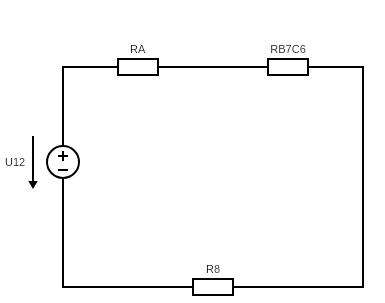
\includegraphics[scale=0.6,keepaspectratio]{fig/Pr1_steps/Pr1_step06.png} \\
\end{center}
\vspace{-0.3cm}

\begin{gather*}
R_{B7C6} = \frac{R_{B7} \times R_{C6}}{R_{B7} + R_{C6}} = \frac{550,8521 \times 1083,5376}{550,8521 + 1083,5376} = 365,1938 \Omega \\\\
\end{gather*}

%%% Krok 7
\begin{center}
\textbf{Krok 7} - Zjednodušíme sériově zapojené rezistory $R_A$, $R_{B7C6}$ a $R_8$ na $R_{EKV}$.
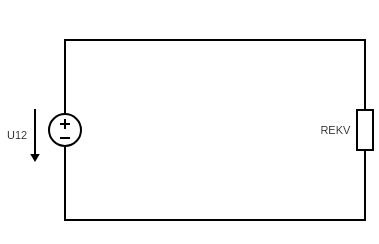
\includegraphics[scale=0.6,keepaspectratio]{fig/Pr1_steps/Pr1_step07.png} \\
\end{center}
\vspace{-0.3cm}

\begin{gather*}
R_{EKV} = R_A + R_{B7C6} + R_8 = 252,5314 + 365,1938 + 265 = 882,7252 \Omega \\\\
\end{gather*}

%%% Krok 8
\begin{center}
\textbf{Krok 8} - Vypočítáme proud.
\end{center}

\begin{gather*}
I = \frac{U_{12}}{R_{EKV}} = \frac{215}{882,7252} = 0,2436 A
\end{gather*}

\newpage

%%% Krok 9
\begin{center}
\textbf{Krok 9} - Zpětně dopočítáme pomocí kroku č. 6 ubýtek napětí na $R_{B7C6}$.
\end{center}

\begin{gather*}
U_{R_{B7C6}} = I \times R_{B7C6} = 0,2436 \times 365,1938 = 88,9612 V \\\\
\end{gather*}

%%% Krok 10
\begin{center}
\textbf{Krok 10} - Když víme, že úbýtek napětí je ve větvích paralelního zapojení stejný tak si můžeme dopočítat proud, který prochází spodní větví.
\end{center}

\begin{gather*}
\boldsymbol{I_{R6}} = I_{R_{C6}} = \frac{U_{R_{B7C6}}}{R_{C6}} = \frac{88,9612}{1083,5376} = \boldsymbol{0,0821 A} \\\\
\end{gather*}

%%% Krok 11
\begin{center}
\textbf{Krok 11} - Dopočítáme úbytek napětí na $R_{6}$.
\end{center}

\begin{gather*}
\boldsymbol{U_{R_6}} = I_{R_6} \times R_{6} = 0,0821 \times 870 = \boldsymbol{71,427 V} \\\\
\end{gather*}